% CREATED BY DAVID FRISK, 2015
\chapter{Introduction}
\hspace{0.25cm}This report provides a brief introduction and usage of PETSc. Portable, Extensible Toolkit for Scientific Computation (PETSc) is a library containing routines useful in the domain of Scientific computing. It uses Message passing interface (MPI) for parallel communications. PETSc contains several libraries(\ref{fig:lib}) which manipulate a set of objects(Vectors,Matrices etc.,). A large number of customizable linear and non linear solvers, Pre-conditioners, time steppers are available at hand to ease the process of scientific code development. 

\begin{figure}[H]
\centering
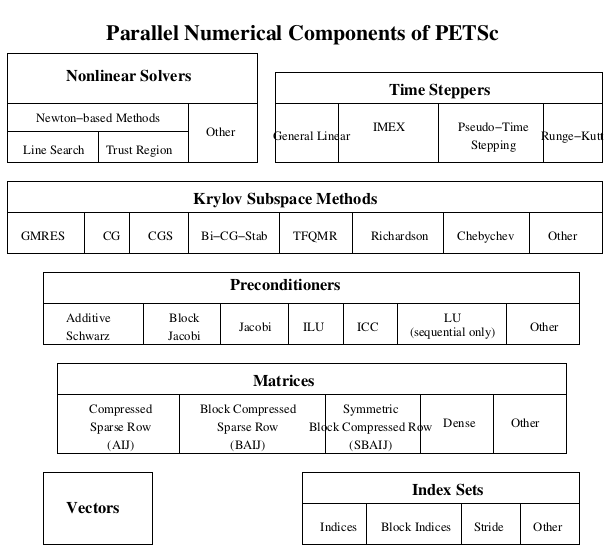
\includegraphics[scale=0.4]{report/figures/library.png}
\caption{Numerical libraries of PETSc \cite{petsc}}
\label{fig:lib}
\end{figure}

\hspace{0.25cm} The succeeding content will describe the implementation of PETSc on a 2D Laplace equation. Further, the code with its accompanying terminologies is briefly explained.  


\section{Laplace equation}
\hspace{0.25cm}The Laplace equation in 2D solved in this code is given below,
\begin{equation}\label{eq:uhe}
 \frac{\partial^2 T}{\partial x^2}+\frac{\partial^2 T}{\partial y^2} = 0
\end{equation}

\hspace{0.25cm}$T$ is any physical variable like Temperature etc., and $x$ and $t$ represent the spatial coordinates.







\section{Numerical Method}
\hspace{0.25cm}The governing equation is discretised using finite difference method and the final equation is expressed below. 

\hspace{0.25cm}A standard 5 point stencil is represented by, 
\begin{figure}[H]
\centering
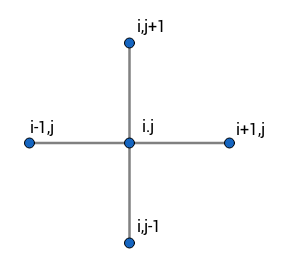
\includegraphics[scale=0.4]{figures/stencil.png}
\caption{five point stencil}
\label{fig:rline}
\end{figure}
\hspace{0.25cm}Using the above representation, the final equation can be written as,
\begin{equation}
\label{eq:fdm}
         T_{i,j}=\frac{1}{4}(T_{i,j+1}+T_{i,j-1}+T_{i,j+1}+T_{i,j-1}) 
\end{equation}

\hspace{0.25cm}This equation is solved with the help of PETSc routines in Fortran programming language. A standard square domain with Dirichlet boundary condition is chosen and Gauss-Seidel iteration method is used for solving.
    


